\documentclass{article}
\usepackage[T1]{fontenc}
\usepackage{lmodern}
\usepackage{graphicx}
\usepackage{amsmath,amssymb}
\usepackage[a4paper,margin=2cm]{geometry}
\usepackage[absolute,overlay]{textpos}
\setlength{\TPHorizModule}{1mm}
\setlength{\TPVertModule}{1mm}
\usepackage[indonesian]{babel}
\usepackage{hyperref}
\setlength{\emergencystretch}{2em}
% unit: Halaman 1

\begin{document}

% === Halaman 1 (llm) ===

\begin{center}
Bahan kuliah IF4020 Kriptografi

{\Huge Elliptic Curve Cryptography (ECC)}

\vspace{110.48mm}

{\Large (Bagian 2)}

\vspace{30mm}

Oleh: Rinaldi Munir

\vspace{10mm}

Program Studi Teknik Informatika\\
Sekolah Teknik Elektro dan Informatika\\
Institut Teknologi Bandung\\
2026
\end{center}

% deskripsi: Ilustrasi geometris penjumlahan titik pada kurva eliptik yang menunjukkan titik P, Q, hasil operasi P*Q, dan hasil refleksi P+Q
% bbox normalisasi: [0.7370, 0.3040, 0.9580, 0.6760]
\begin{textblock*}{46.41mm}(154.77mm,90.29mm)
\noindent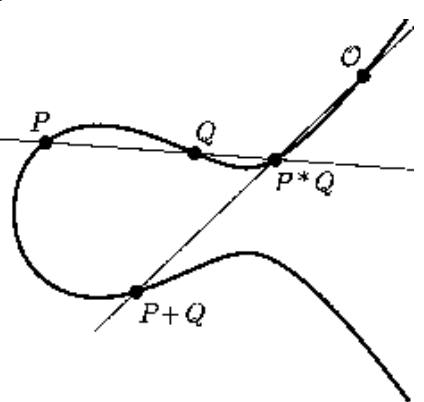
\includegraphics[width=46.41mm,height=110.48mm]{../../images/llm/page_001_img_01.png}%
\end{textblock*}

\end{document}
